\documentclass[full]{l3doc}

\usepackage{fontspec}
\usepackage{biblatex}
\addbibresource{literatur.bib}

\usepackage{codeanatomy}
\usepackage{listings}
\lstset {
    basicstyle=\small\ttfamily
    ,escapeinside={!}{!}
    ,resetmargins=true
    ,columns=fullflexible
}

\def\thinmargin{\list{}{\rightmargin-30pt\leftmargin-70pt}\item[]}
\let\endthinmargin=\endlist

% others shortcuts
\newcommand{\slsh}{\textbackslash{}}
\newcommand{\TikZ}{Ti\textit{k}Z}
\newcommand{\inputlisting}[1]{%
\lstinputlisting[%
    xleftmargin=-70pt
    ,resetmargins=true
    ,escapeinside={}{}
    ]{#1} %    
}
\usepackage{hyperref}

\author{Hồng-Phúc Bùi}
\title{Usage of \pkg{codeanatomy} in conjunction with \pkg{listings}}
\date{Sommer 2019}




\begin{document}

\maketitle

\section{General Usage in Conjuntion with Package \pkg{listings}}
\subsection{Setup Package \pkg{listings}}
The most important setup for the package \pkg{listings} is the delimiter to escape \LaTeX{}
commands in Listing. With this escape delimiter we can mark a piece of code as with |\cPart|.
In this example we use |!| and |!| as delimiter. Code between |!| and |!| is evaluated as 
\LaTeX{}-code.

\lstset {    
    escapeinside={+}{+}
}
\begin{thinmargin}
\begin{tikzpicture}[remember picture]
% {[on background layer]\draw[code grid debug] (-3.5,-0.5) grid (5.5,4.5);}
\node(code) [anatomy] at (0,0){%
\begin{lstlisting}
\usepackage{codeanatomy}
\usepackage{listings}
\lstset {
   basicstyle=\small\ttfamily
  ,escapeinside=+\cPart{delimiter}{\{!\}\{!\}}+
}
\end{lstlisting}
};
\codeAnnotation{delimiterText} (4,-0.5) {Setup \texttt{!} and \texttt{!}\\as delimiter}

\draw[->, annotation] (delimiterText) -- (delimiter);
\end{tikzpicture}
\end{thinmargin}


Delimiter can also be reset in |document|-Environment, typical just before a new \verb:\begin{lstlisting}:
environment so each anatomy can have different delimiter. The fact is, in this document I use |+| and |+| for 
the above listing, so that I can typeset |!| in this listing.

\subsection{Typeset Code}
The command |\codeBlock| does not work if the environment |lstlisting| is passed to its argument. So instead of 
|\codeBlock| we must use the \TikZ{} command |\node|:

\begin{thinmargin}
\begin{tikzpicture}[remember picture]    
\node(code) [anatomy] at (0,0) {
\begin{lstlisting}
\begin{tikzpicture}[remember picture]
+\cPart{tikzNode}{\slsh{}node(code) [anatomy] at (0,0)}+ {
+\cPart{listingBegin}{\texttt{\slsh{}begin\{lstlisting\}}}\vspace{1.5pt}+
+\extremPoint{mostLeft}[most top]+function gcd(p,q) {
    if (q === 0) {
        return q;                
    }else{
        let r = p % q;
        return gcd(q, r);+\extremPoint{mostRight}+
    }
}+\extremPoint{mostBottom}[most bottom]+
+\cPart{listingEnd}{\texttt{\slsh{}end\{lstlisting\}}}+
}+\cPart{semiColon}{;}+
\end{tikzpicture}
\end{lstlisting}
};

\fitExtrem{listingContent}{(mostLeft) (mostRight) (mostBottom)}

% Annotations
\codeAnnotation{tikzNodeText} (-2, 5.5)      {use \texttt{\slsh{}node}\\instead of\\\texttt{\slsh{}codeBlock}}
\codeAnnotation{listingText}  (-2, 3)        {typeset code\\in\\\texttt{lstlisting}\\environment}
\codeAnnotation{listingContentText} (6.5, 3) {whitespaces\\in code\\are kept}
\codeAnnotation{semiColonText} (6.5, 0.6)  {don't forget\\semicolon}

% Arrows from labels to code parts
\draw[->,annotation] (tikzNodeText) -- (tikzNode.west);
\draw[->,annotation] (listingText) -- (listingBegin.west);
\draw[->,annotation] (listingText) -- (listingEnd.west);
\draw[->,annotation] (listingContentText) -- (listingContent);
\draw[->,annotation] (semiColonText) -- (semiColon);
\end{tikzpicture}
\end{thinmargin}

Figure~\ref{fig:full-formatted-code} shows result of the above code.

\begin{figure}[ht]
\centering    
\begin{tikzpicture}[remember picture]
\node(code) [anatomy] at (0,0) {
\begin{lstlisting}
function gcd(p,q) {
    if (q === 0) {
        return q;
    }else{
        let r = p % q;
        return gcd(q, r)
    }
}
\end{lstlisting}
};
\end{tikzpicture}
\caption{Code Listing is formatted\label{fig:full-formatted-code}}
\end{figure}

\subsection{Mark Code}
% --------------------

The command |\cPart| can be used to mark single-line code parts. For 
multiple-line code parts once can use |\extremPoint| to mark the outer most 
points of code parts and |\fitExtrem| to cover exterm points of a code part.
These commmands must be put in delimiter, here |!| and |!|.

\begin{thinmargin}
\begin{tikzpicture}[remember picture]    
\node(code) [anatomy] at (0,0) {
\begin{lstlisting}
\begin{tikzpicture}[remember picture]
\node(code) [anatomy] at (0,0) {
+\texttt{\slsh{}begin\{lstlisting\}}+    
!\cPart{fnHead}{function \cPart{fnName}{gcd}\cPart{paramList}{(p,q)}}! {
    +\cPart{ep1}{!\slsh{}extremPoint\{mostLeft\}[most top]!}+if (q === 0) {
        return q;                
    }else{
        +\cPart{cp}{!\slsh{}cPart\{localVar\}\{let r\}!}+ = p % q;
        return gcd(q, r);+\cPart{ep2}{!\slsh{}extremPoint\{mostRight\}!}+
    }+\cPart{ep3}{!\slsh{}extremPoint{mostBottom}[most bottom]!}+
}
+\texttt{\slsh{}end\{lstlisting\}}+
};
\fitExtrem{fnBody}{(mostLeft) (mostRight) (mostBottom)}
\end{tikzpicture}
\end{lstlisting}
};
% Annotations
\codeAnnotation{epText} (11,2.5) {\texttt{extremPoint}-s mark\\outer most\\of the function body}
\codeAnnotation{cpText} (-2,3) {\texttt{cPart} marks a\\single line\\code part}
% Arrows
\draw[->,annotation] (epText) -- (ep1.south east);
\draw[->,annotation] (epText) -- (ep2.east);
\draw[->,annotation] (epText) -- (ep3.south east);
\draw[->,annotation] (cpText) -- (cp);
\end{tikzpicture}
\end{thinmargin}

Figure~\ref{fig:listing-code-parts} shows the result of the above code.

\begin{figure}[ht]
\centering
\lstset{escapeinside={!}{!}}
\begin{tikzpicture}[remember picture]
\node(code) [anatomy] at (0,0) {
\begin{lstlisting}
!\cPart{fnHead}{function \cPart{fnName}{gcd}\cPart{paramList}{(p,q)}}! {
    !\extremPoint{mostLeft}[most top]!if (q === 0) {
        return q;
    }else{
        !\cPart{localVar}{let r}! = p % q;
        return gcd(q, r);!\extremPoint{mostRight}!
    }!\extremPoint{mostBottom}[most bottom]!
}
\end{lstlisting}
};
\fitExtrem{fnBody}{(mostLeft) (mostRight) (mostBottom)}
\end{tikzpicture}
\caption{Code Listing with mark of code parts\label{fig:listing-code-parts}}
\end{figure}

\subsection{Add Annotations to Listing}
% -------------------------------------
This step is the same as the description in the main document of package \pkg{codeanatomy}.
Readers can typeset annotations to the above listing like an exercise.






\section{Some examples}
% ====================
% Reset to standard

Most of examples in this section are redrawn from the textbook~\autocite{sedgewick_wayne_2016}.

\subsection{Anatomy of a Java Program~\autocite[5]{sedgewick_wayne_2016}}
% -----------------------------------
\begin{thinmargin}
\inputlisting{java-program.tex}
\end{thinmargin}

\lstset{escapeinside={!}{!}}
\begin{tikzpicture}[remember picture]
\node(code) [anatomy] at (0,0){%
\begin{lstlisting}
public !\iPart{class}{class}! !\cPart{className}{HelloWorld}!
{
    !\extremPoint{mainLeft}[most top]!public static void main(String[] argv)
    {
        !\extremPoint{left}[most top]\iPart{assign}{
          \bgcode{// Prints "Hello World" in the terminal window}}
          \extremPoint{fnR} \extremPoint{mR}!
        !\iPart{fnCall}{System.out.print( "Hello World");}\extremPoint{mostBottom}[most bottom]!
    }!\extremPoint{mainBottom}[most bottom]!
}
\end{lstlisting}
};

\fitExtrem{classBody}{(mainLeft) (mR) (mainBottom)}
\fitExtrem{functionBody}{(left) (fnR) (mostBottom)}


\codeAnnotation{fileNameText} (1.5,5) {text file named \texttt{HelloWorld.java}}
\codeAnnotation{classNameText} (3.5,4.25) {name}
\codeAnnotation{classBodyText} (6.5,3.6) {\texttt{main()} method}
\codeAnnotation{functionBodyText} (2.5,-0.5) {body}
\codeAnnotation{statement} (8,0) {statements}

\draw[->,annotation] (fileNameText) -- (class);
\draw[->,annotation] (classNameText) -- (className);
\draw[->,annotation] (classBodyText.south west) -- (classBody);
\draw[->,annotation] (functionBodyText) -- (functionBody);
\draw[->,annotation] (statement) -- (assign.353);
\draw[->,annotation] (statement) -- (fnCall.350);
\end{tikzpicture}


\subsection{Anatomy of an expression~\autocite[17]{sedgewick_wayne_2016}}
% -----------------------------------
\begin{thinmargin}
    \inputlisting{java-expression.tex}
\end{thinmargin}

\lstset{escapeinside={!}{!}}
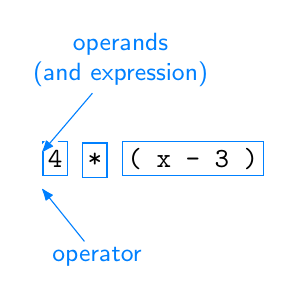
\begin{tikzpicture}[remember picture]    
\codeBlock{\cPart{op1}{4} \cPart{op}{*} \cPart{op2}{( x - 3 )} }

\codeAnnotation{operand}  (1,1.5) {operands\\(and expression)}
\codeAnnotation{operator} (0.7,-1) {operator}

\draw[->,annotation] (operand) -- (op1.north);
\draw[->,annotation] (operand) -- (op2.north);
\draw[->,annotation] (operator) -- (op.south);
\end{tikzpicture}


\subsection{Using a primitive Data Type~\autocite[17]{sedgewick_wayne_2016}}
% -------------------------------------

\subsection{Anatomy of a method signature~\autocite[30]{sedgewick_wayne_2016}}
% ---------------------------------------

\subsection{Using a library method~\autocite[30]{sedgewick_wayne_2016}}
% --------------------------------

\subsection{Anatomy of an \texttt{if} statement~\autocite[51]{sedgewick_wayne_2016}}
% ---------------------------------------------

\subsection{Anatomy of a \texttt{while} loop~\autocite[54]{sedgewick_wayne_2016}}
% ------------------------------------------

\subsection{Anatomy of a \texttt{for} loop~\autocite[59]{sedgewick_wayne_2016}}
% ----------------------------------------

\subsection{Anatomy of a static method~\autocite[196]{sedgewick_wayne_2016}}
% ----------------------------------------
\end{document}

